\documentclass{beamer}
%\usepackage{beamerarticle}
\usepackage{heppennames}
\usepackage{hepnicenames}
\usepackage{graphicx} 
\usepackage{multirow}
\usepackage{amsbsy,amsmath,amssymb}
\usepackage{booktabs}
% ********** Styl prezentacji **********
\mode<presentation>
{
	\usetheme{Singapore}
  \setbeamercovered{transparent}
   \setbeamertemplate{footline}[frame number] 
%   \setbeamertemplate{navigation symbols}{ 
%   \insertslidenavigationsymbol
%   \insertframenavigationsymbol
%   \insertsubsectionnavigationsymbol
%   \insertsectionnavigationsymbol
%   \insertdocnavigationsymbol
%   \insertbackfindforwardnavigationsymbol
%   \hskip 0.3cm
%   %\insertframenumber / \inserttotalframenumber  % <<< frame #
%   %\insertpagenumber / \insertpresentationendpage % <<< page #
% } 
}

\usepackage[english]{babel}
\usepackage[latin1]{inputenc}

% font definitions, try \usepackage{ae} instead of the following
% three lines if you don't like this look
\usepackage{mathptmx}
\usepackage[scaled=.90]{helvet}
\usepackage{courier}


\usepackage[T1]{fontenc}

\author{S. Poss for the CERN LCD group}
\institute[CERN]{CERN}

\subject{CLICCDR}
\AtBeginSection[]
{   
{
    \usebackgroundtemplate{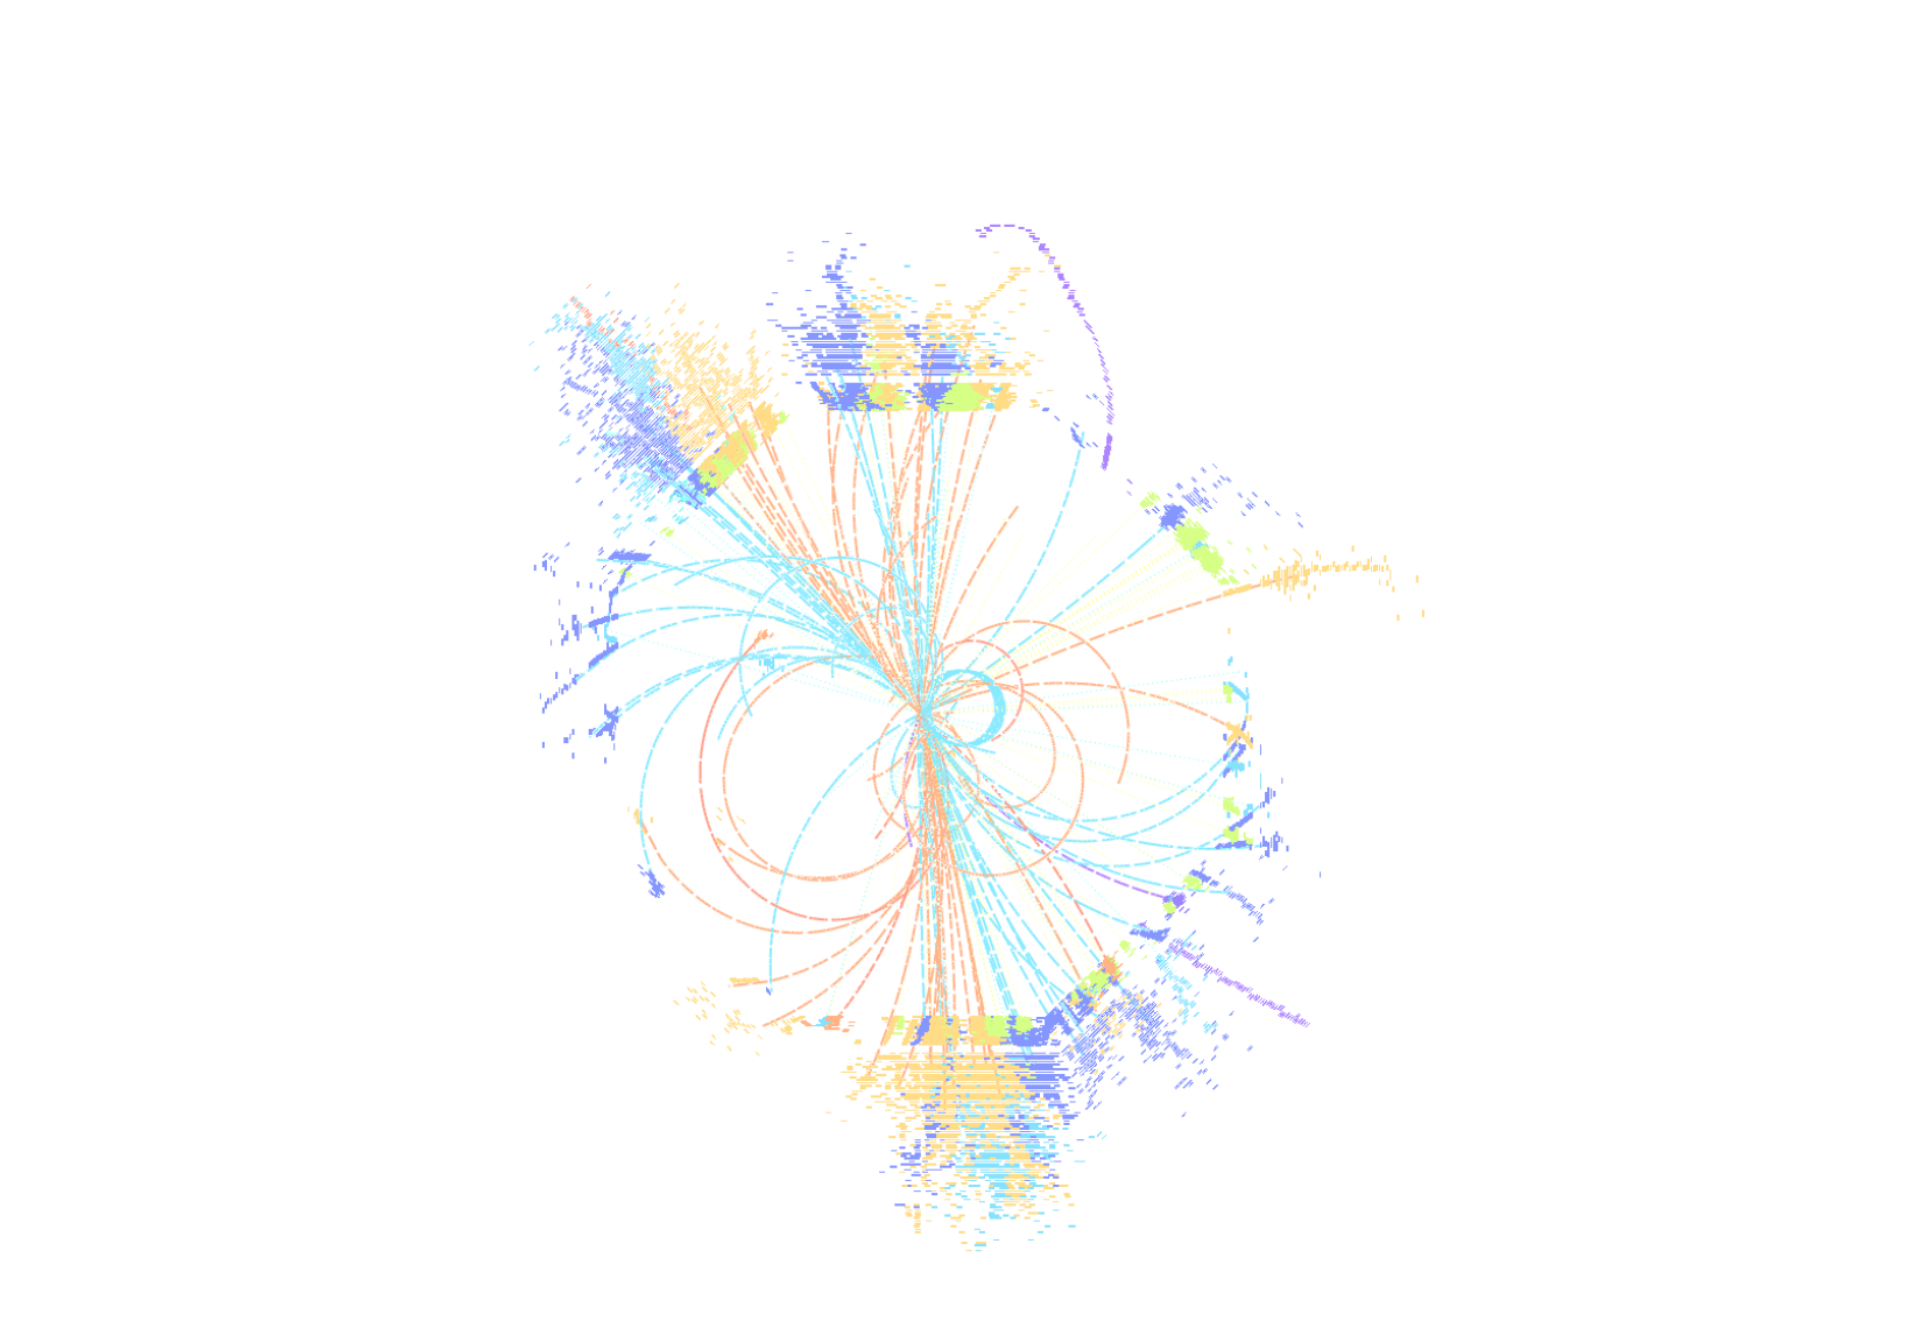
\includegraphics[width=\paperwidth]{background.png}}
	\begin{frame}<beamer>
		\frametitle{Outline}
		\tableofcontents[currentsection,currentsubsection]
	\end{frame}
}
}
\title[]{CLIC Physics and detectors CDR}
%%\subtitle{Our experience}

\date{\today}

\begin{document}

{
\usebackgroundtemplate{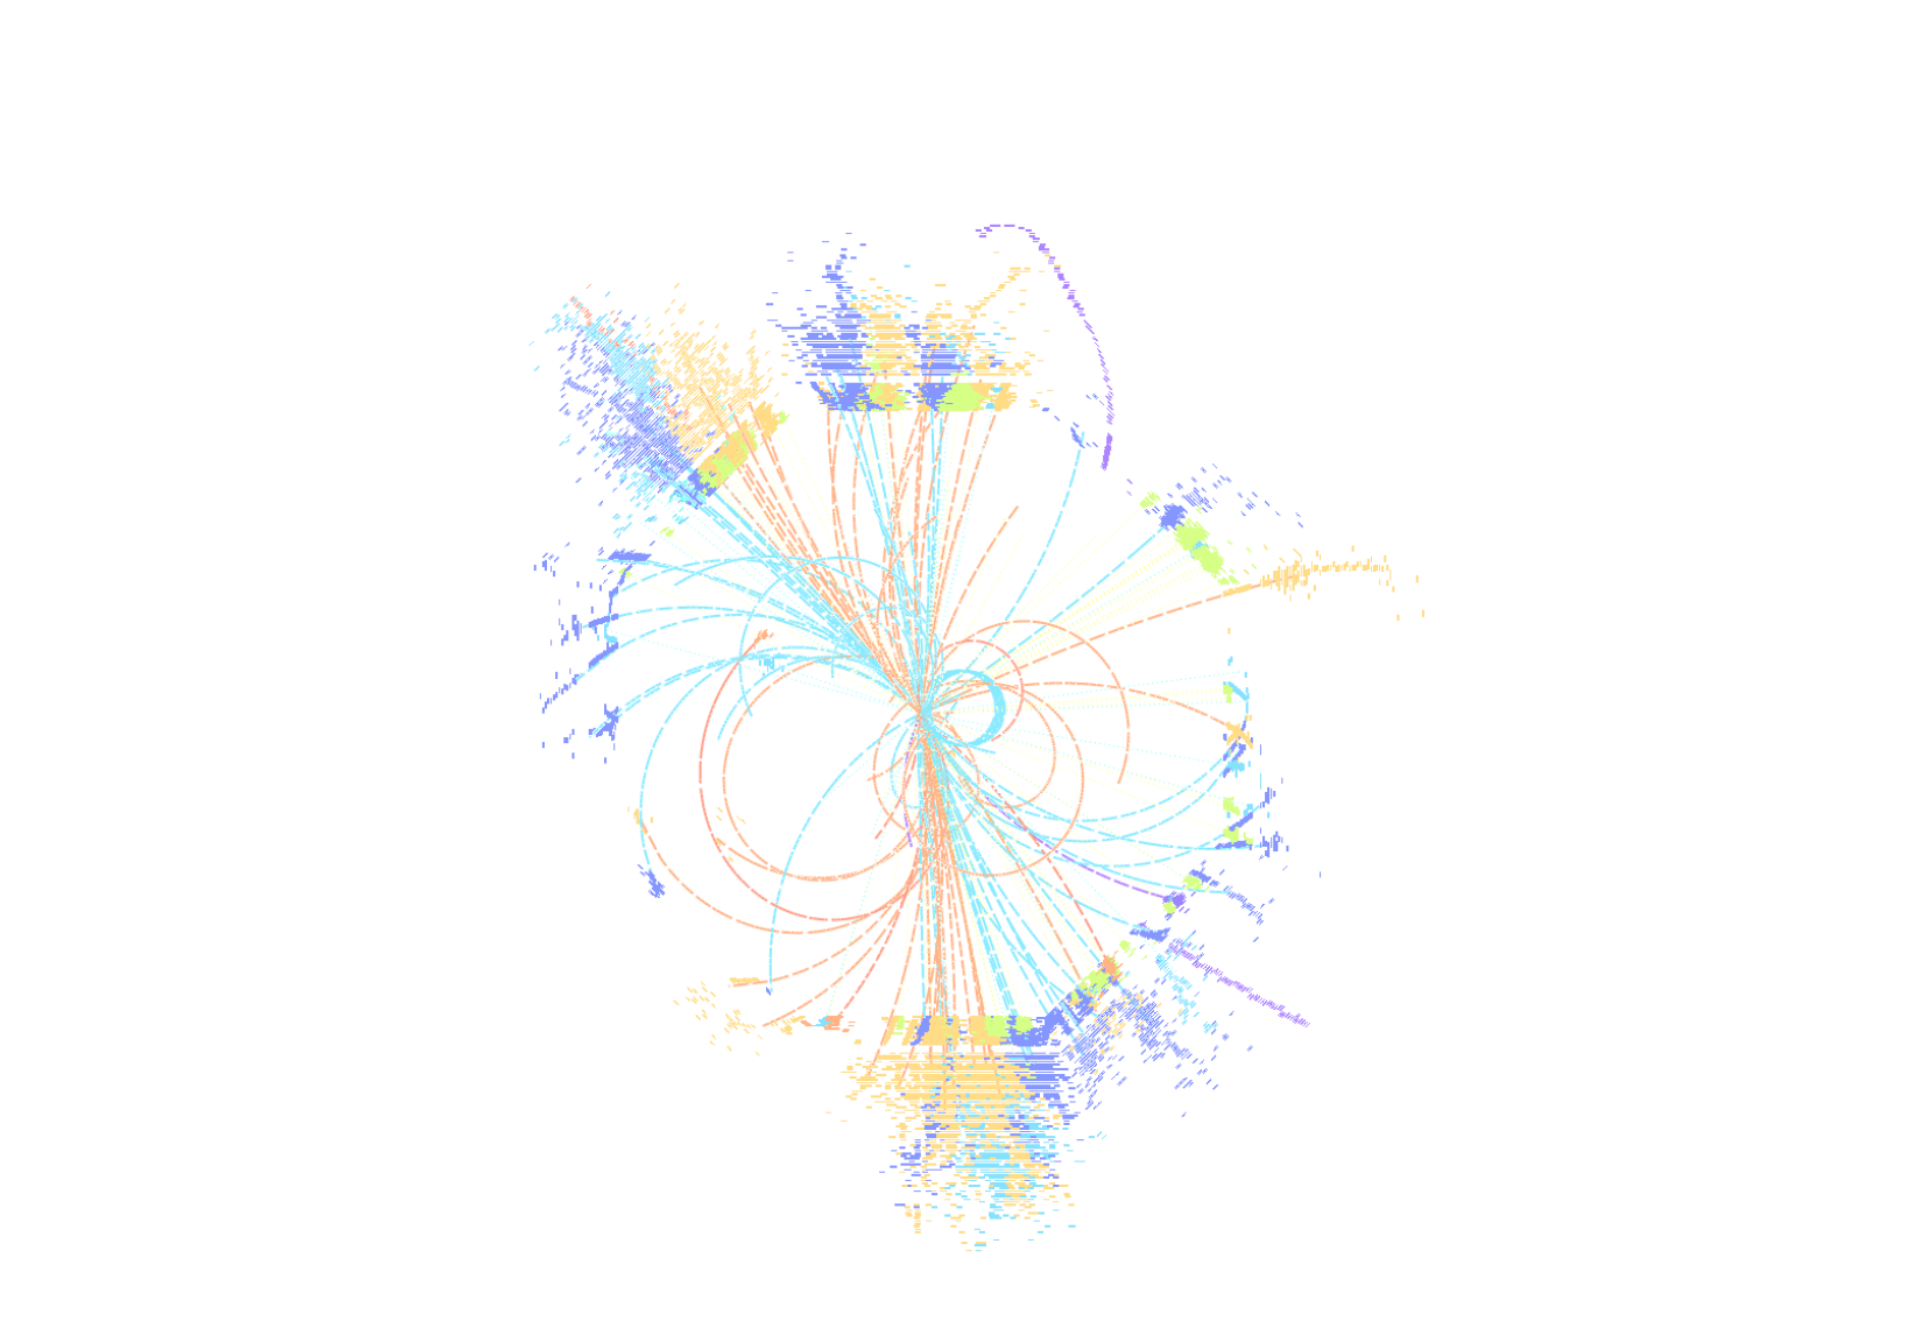
\includegraphics[width=\paperwidth]{background.png}}

\begin{frame}
	\titlepage
\end{frame}

\begin{frame}
\frametitle{Outline}
\tableofcontents
% You might wish to add the option [pausesections]
\end{frame}
}

\section[Motivations for CLIC]{Motivations for a CLIC machine}%1slide
\begin{frame}
 \frametitle{Motivations for a CLIC machine}
 CLIC: Compact LInear Collider, 3TeV design energy
 \begin{itemize}
   \item Complementary to LHC
   \item In case of discoveries: precision Higgs physics, SUSY studies, etc.
 \end{itemize}
 
\end{frame}

\section{Physics Potential}
\begin{frame}
\frametitle{SM Higgs}

\end{frame}
\begin{frame}
\frametitle{BSM Higgs}
\end{frame}
\begin{frame}
\frametitle{SUSY}
\end{frame}
\begin{frame}
\frametitle{Other studies and summary}

\end{frame}

\section[CLIC]{The CLIC Machine}
\begin{frame}
\frametitle{Technology}

\end{frame}
\begin{frame}
\frametitle{Machine properties}

\end{frame}
\begin{frame}
\frametitle{Machine Detector Integration}
QD0 is IN the detector, stabilization
\end{frame}

\begin{frame}
\frametitle{Machine induced backgrounds}

\end{frame}

\section[Detectors]{The Detectors}
\begin{frame}
\frametitle{Required perfomance}

\end{frame}
\begin{frame}
\frametitle{Overview}
\end{frame}
\begin{frame}
\frametitle{Vertex detector optimization}
\end{frame}

\begin{frame}
\frametitle{Tracking in SiD}

\end{frame}
\begin{frame}
\frametitle{Tracking in ILD}
\end{frame}
\begin{frame}
\frametitle{ECAL}
\end{frame}
\begin{frame}
\frametitle{HCAL}
Use tungsten for lower depth
\end{frame}
\begin{frame}
\frametitle{CALICE results}
\end{frame}

\section[Bkg treatment]{Dealing with the machine induced background}
\begin{frame}
\frametitle{Timing cuts}
\end{frame}
\begin{frame}
\frametitle{Jet reconstruction}
\end{frame}

\section{Physics Results}
\begin{frame}
 \frametitle{Benchmark channels}
\end{frame}
\begin{frame}
\frametitle{SM Higgs}
\end{frame}
\begin{frame}
\frametitle{SM Higgs}
\end{frame}
\begin{frame}
\frametitle{Squarks}
\end{frame}
\begin{frame}
\frametitle{Squarks}
\end{frame}
\begin{frame}
\frametitle{Sleptons}
\end{frame}
\begin{frame}
\frametitle{Sleptons}
\end{frame}
\begin{frame}
\frametitle{Gauginos}
\end{frame}
\begin{frame}
\frametitle{Gauginos}
\end{frame}
\begin{frame}
\frametitle{Heavy Higgs}
\end{frame}
\begin{frame}
\frametitle{Top physics at 500GeV: vertex detector}
\end{frame}
\begin{frame}
\frametitle{Top physics at 500 GeV: compare with ILC}
\end{frame}

\section{Conclusion}
\begin{frame}
\frametitle{Overview}
\end{frame}
\begin{frame}
\frametitle{Signatory list}
\end{frame}
\appendix

\section{Software}
\begin{frame}
\frametitle{Generation}
\end{frame}
\begin{frame}
\frametitle{Simulation}
\end{frame}
\begin{frame}
\frametitle{Handling background in the software}
\end{frame}
\begin{frame}
\frametitle{Reconstruction}
\end{frame}
\begin{frame}
\frametitle{Using the GRID: ILCDIRAC}
\end{frame}

\end{document}